\subsubsection{Results}
\paragraph{} The results first five blocks of the darpa and airforce are shown in Table 1 and Table 2.
\begin{table}
\centering
\begin{tabular}{|c|c|c|c|c|}
    \hline
        Dataset & k & Dimension & Mass & Density \\
    \hline
        Darpa & 1 & 2 X 1 X 47 & 278288 & 16697.3 \\
    \hline
        Darpa & 2 & 8 X 3 X 118 & 688245 & 16005.7 \\
    \hline
        Darpa & 3 & 2 X 1 X 44 & 230124 & 14688.8 \\
    \hline
        Darpa & 4 & 1 X 1 X 5 & 26371 & 11301.8 \\
    \hline
        Darpa & 5 & 2 X 1 X 18 & 77425 & 11060.7 \\
    \hline
\end{tabular}
\caption {Top 5 dense blocks for Darpa Dataset}
\end{table}

\begin{table}
\centering
\begin{tabular}{|c|c|c|c|c|}
    \hline
        Dataset & k & Dimension & Mass & Density \\
    \hline
        Airforce & 1 & 1x1x1x1x1x1x1 & 1930307 & 1930307 \\
    \hline
        Airforce & 2 & 1x1x1x2x1x2x2 & 2532845 & 421776.6 \\
    \hline
        Airforce & 3 & 3x4x3x3x1x58x21 & 554067 & 41704.0\\
    \hline
        Airforce & 4 & 3x4x3x13x4x67x35 & 493873 & 25691.3 \\
    \hline
        Airforce & 5 & 1x1x3x1x1x36x20 & 168929 & 18769.9 \\
    \hline
\end{tabular}
\caption {Top 5 dense blocks for Airforce Dataset}
\end{table}

\subsubsection{Suspiciousness Analysis}
I write a program to count how many tuples found in block are labelled as not normal connections and I found in most blocks almost all tuples in those blocks are tagged as ``attack''. It shows that the approach is effective. 

\subsubsection{ROC and AUC}
The ROC Curve and the AUC value are shown in Figure 1 and Figure 2.
\begin{figure}
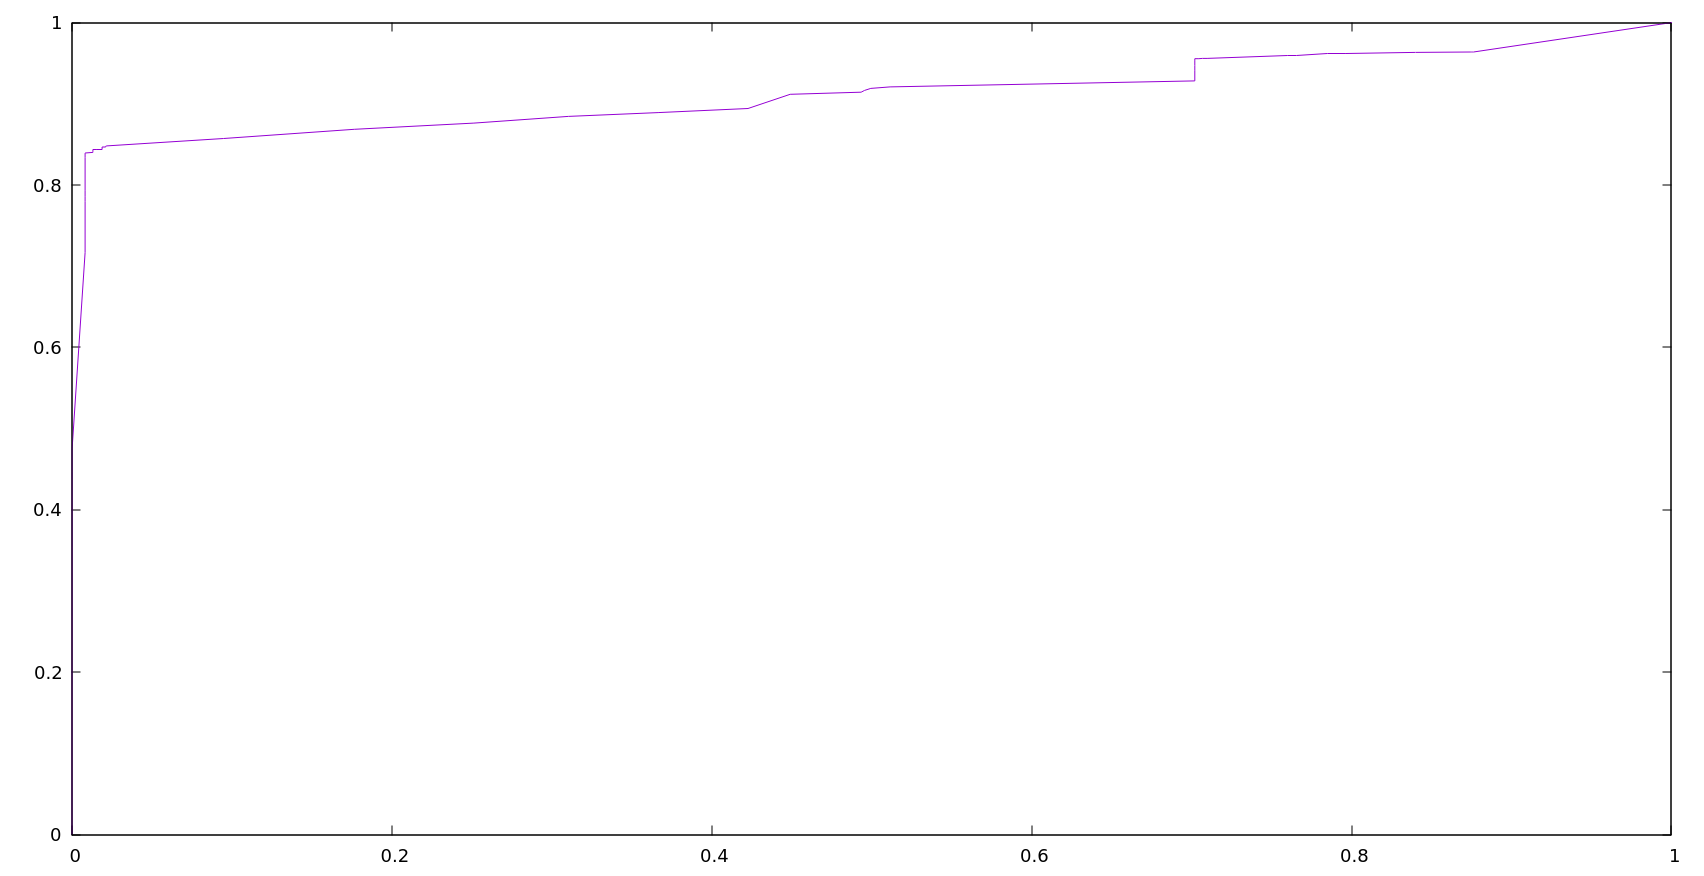
\includegraphics[scale=0.5]{roc1.png}
\caption{ROC Curve of Darpa Dataset After 60-Block Detections, AUC = 0.912}
\end{figure}

\begin{figure}
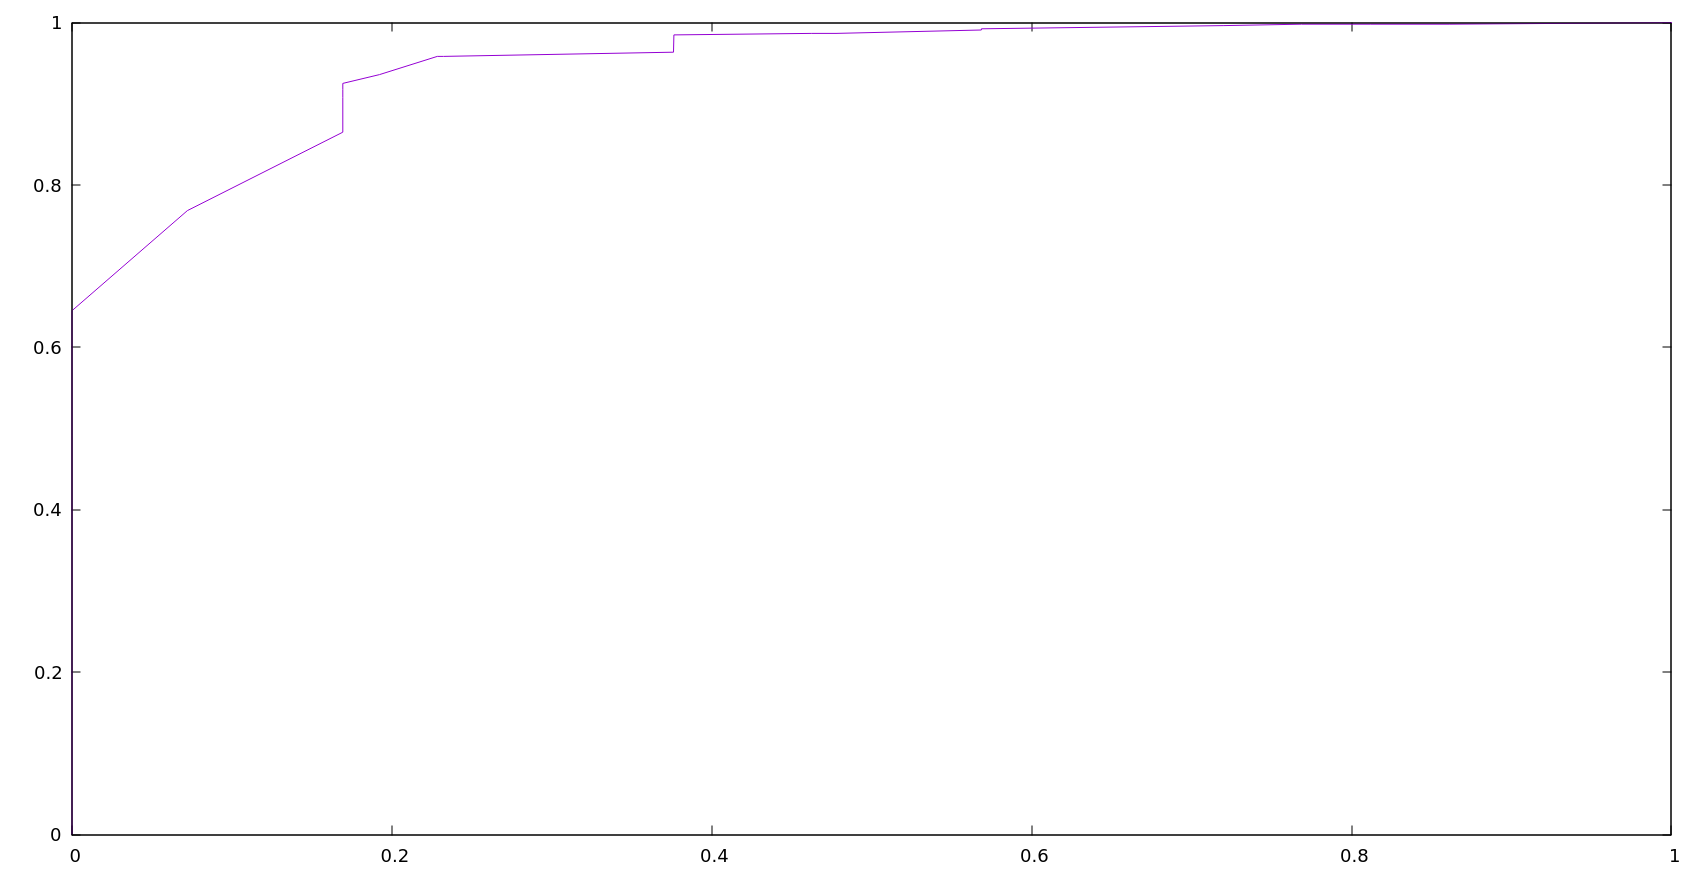
\includegraphics[scale=0.5]{roc2.png}
\caption{ROC Curve of Airforce Dataset After 20-Block Detections, AUC = 0.948}
\end{figure}